\addtocontents{toc}{\vspace{1em}}
\chapter{Conclusions}\label{chap:conclusion}

\lettrine[findent=.3em,lines=2,nindent=-0.4em]{T}{he} central research topic of this thesis was the correctness of services and their compositions. We investigated several scenarios of service-oriented computing (\acronym{SOC}) and defined formalizations, correctness notions, and verification algorithms. In this chapter, we provide a summary of the contributions and discuss the theoretical and practical limitations of the results presented. We conclude the thesis by sketching directions for future extensions of the contributions of this thesis.





%%%%%%%%%%%%%%%%%%%%%%%%%%%%%%%%%%%%%%%%%%%%%%%%%%%%%%%%%%%%%%%%%%%%%%%%%%%%%%
\section{Summary of contributions}
%%%%%%%%%%%%%%%%%%%%%%%%%%%%%%%%%%%%%%%%%%%%%%%%%%%%%%%%%%%%%%%%%%%%%%%%%%%%%%

We approached correctness of \acronym{SOC} from three different directions, each investigated in a separate part of this thesis. In the following, we briefly summarize the contributions of this thesis.




%%%%%%%%%%%%%%%%%%%%%%%%%%%%%%%%%%%%%%%%%%%%%%%%%%%%%%%%%%%%%%%%%%%%%%%%%%%%%%
\subsection*{Correctness of services}

A fundamental correctness criterion for services is controllability. The presence of interaction partners is a necessary requirement for a service to be used in any service composition. In this thesis, we extended controllability in two aspects.

\enlargethispage*{\baselineskip}

\begin{niceitemize}
\item In \autoref{chap:validation}, we presented a refinement of controllability. Using behavioral constraints, the set of all potential interaction partners can be restricted to only those partners which additionally satisfy specified properties. We formalized behavioral constraints with constraint automata and product operators and extended the respective tools. As behavioral constraints are very flexible, they can be used in a variety of scenarios, ranging from service validation to service construction.

\item \Autoref{chap:diagnosis} extended the controllability analysis algorithm with the ability to generate counterexamples in case a service is uncontrollable. We first discussed various design flaws which can render a service uncontrollable and showed that it is not possible to derive antipatterns to check and diagnose uncontrollability on the structure of a service. Consequently, we presented several modifications of the controllability algorithm and introduced a diagnosis approach to construct a counterexample.
\end{niceitemize}




%%%%%%%%%%%%%%%%%%%%%%%%%%%%%%%%%%%%%%%%%%%%%%%%%%%%%%%%%%%%%%%%%%%%%%%%%%%%%%
\subsection*{Correctness of service compositions}

A service composition should behave similar to a monolithic system; that is, distribution aspects should not change the functionality in an undesirable manner. To this end, correctness of service compositions can be expressed with classical requirements such as absence of deadlocks and boundedness of the system. Conceptually, correctness of service compositions can be verified using existing state-of-the-art checking techniques. To support the \emph{design} of correct service compositions, this thesis makes three contributions in this area.

\begin{niceitemize}
\item In \autoref{chap:verification}, we formalized with \acronym{WS-BPEL} and \bpelchor{} industrial service specification languages to make the verification techniques directly applicable to industrial service models. We showed that compatibility can be verified for large service compositions, because existing state space reduction techniques are effective in the setting of complete service compositions; that is, closed systems.

\item We applied verification techniques presented in the first part of this thesis to support the design of service compositions. By treating an incomplete service composition as a single service with an interface to missing participants, we can check controllability of this service to synthesize a ``communication skeleton'' of the missing participants which is by construction compatible to the other participants.

\item In \autoref{chap:correction}, we presented techniques to automatically derive recommendations on how to correct incompatible service choreographies. Unlike the previous completion approach, the correction algorithm additionally takes the incorrect service model into account to derive minimal invasive edit actions.
\end{niceitemize}




%%%%%%%%%%%%%%%%%%%%%%%%%%%%%%%%%%%%%%%%%%%%%%%%%%%%%%%%%%%%%%%%%%%%%%%%%%%%%%
\subsection*{Correctness of service choreographies}

As an alternative to create large systems by composing existing services, service choreographies have been introduced to specify the behavior of a service composition from a global perspective. Realizability of such specifications has already been studied in terms of various formalisms. In this thesis, we presented three contributions to realizability of choreographies.

\begin{niceitemize}
\item We defined a hierarchy of realizability notions. The novel concept of \emph{distributed realizability} complements existing notions, and it turns out that many examples from literature, which are not realizable in the classical sense, are in fact distributedly realizable.

\item We linked choreography realization to decentralized controllability~\cite{Wolf_2008_topnoc}. This relationship not only allows us to reuse an existing algorithm to remove unrealizable conversations from a choreography specification, but it also facilitates the application of other techniques of this thesis, for instance behavioral constraints to refine choreography models.

\item By defining choreographies with service automata, both synchronous and asynchro\-nous communication are first-class citizens. This allows us to study choreography realization in the context of both communication paradigms.
\end{niceitemize}





%%%%%%%%%%%%%%%%%%%%%%%%%%%%%%%%%%%%%%%%%%%%%%%%%%%%%%%%%%%%%%%%%%%%%%%%%%%%%%
\section{Classification of contributions}
%%%%%%%%%%%%%%%%%%%%%%%%%%%%%%%%%%%%%%%%%%%%%%%%%%%%%%%%%%%%%%%%%%%%%%%%%%%%%%

The previous section summarized the contributions with respect to the point of view on a service-oriented system. For each scenario, we made contributions toward the ultimate goal of correct systems which are composed of interacting services. In this section, we classify the contributions alongside with the topics which we discussed in the introduction of this thesis, see \autoref{fig:classificationresults}. {\em This classification is not specific to \acronymit{SOC}, but can be seen as a general roadmap to achieve correctness in other domains.}

%%%%%%%%%%%%%%%%%%%%%%%%%%%%%%%%%%%%%%%%%%%%%%%%%%%%%%%%%%%%%%%%%%%%%%%%%%%%%%
\begin{figure}
\centering
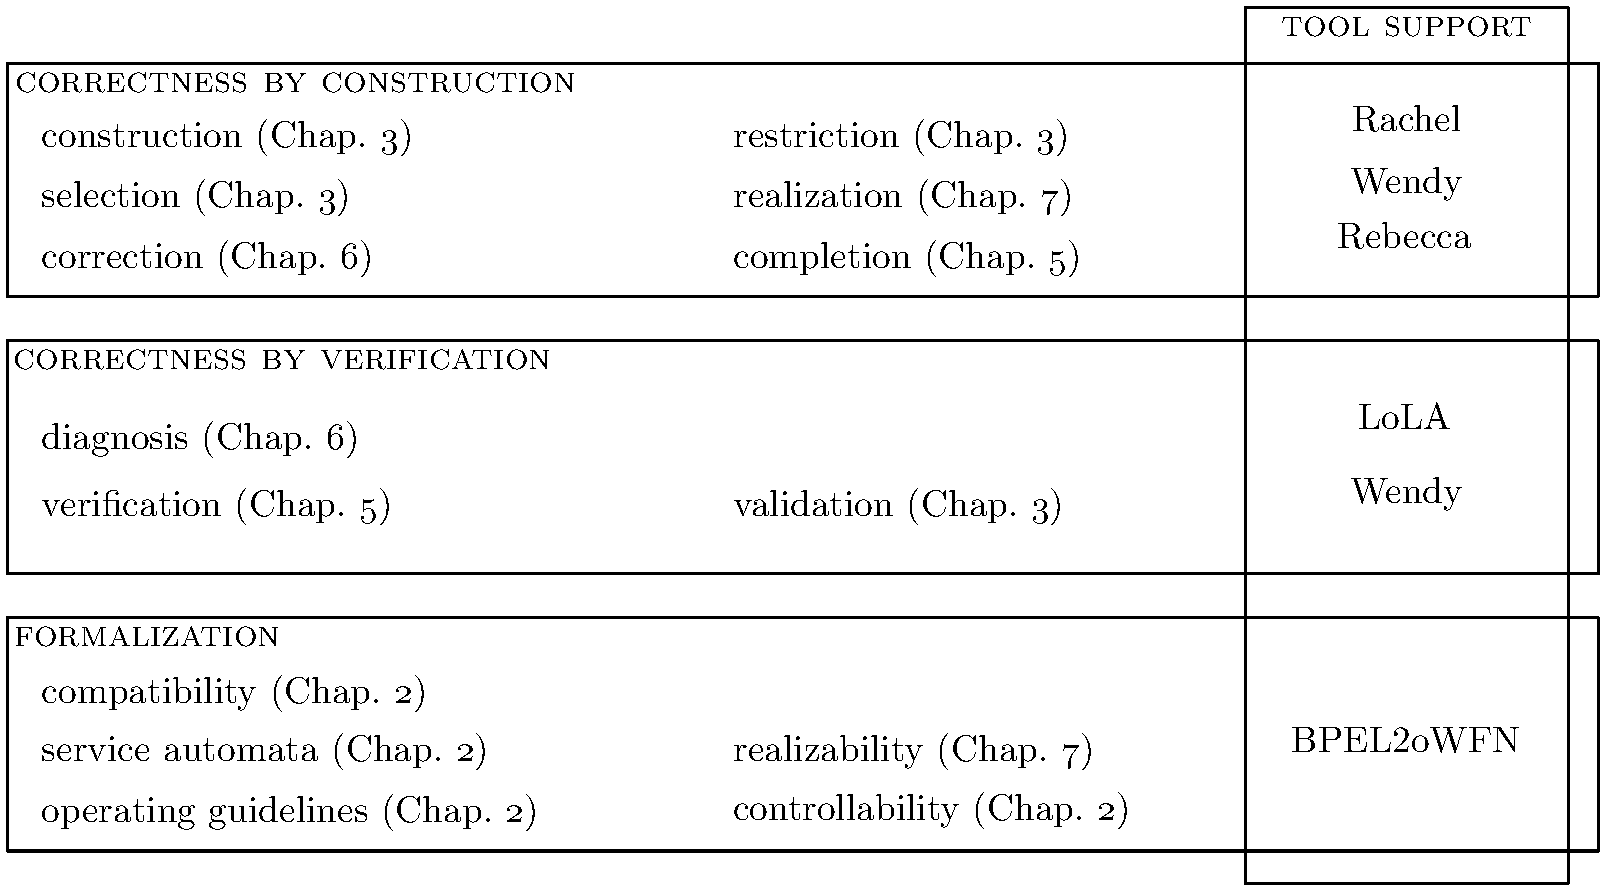
\includegraphics[scale=0.4]{conclusion/results}
\caption{Classification of the thesis' contributions.}\label{fig:classificationresults}
\end{figure}
%%%%%%%%%%%%%%%%%%%%%%%%%%%%%%%%%%%%%%%%%%%%%%%%%%%%%%%%%%%%%%%%%%%%%%%%%%%%%%




%%%%%%%%%%%%%%%%%%%%%%%%%%%%%%%%%%%%%%%%%%%%%%%%%%%%%%%%%%%%%%%%%%%%%%%%%%%%%%
\subsection*{Formalization}

We formalized the relevant aspects of services with a \emph{single mathematical formalism}: service automata. The formalization is not only a prerequisite to formally reason about services and to apply verification techniques, but also makes the results independent of specific service description languages. Using a simple formalism consisting only of states, transitions, and an interface, upcoming and existing languages are likely to be canonically translated into service automata. We only briefly sketched the translation of \acronym{WS-BPEL} and \bpelchor{} in this thesis, but also more complex features of such languages can be translated in a straightforward manner~\cite{LohmannVD_2008_topnoc}.

\emph{The choice of a single formalism can not be stressed enough.} We used service automata to model single services, incomplete and complete service compositions, and service choreographies; that is, all aspects of \acronym{SOC} we studied in this thesis. This allowed us to naturally apply advanced techniques without the need to refine all results for different questions. Additionally, the choice of only once formalism also simplified the development of software tools.




%%%%%%%%%%%%%%%%%%%%%%%%%%%%%%%%%%%%%%%%%%%%%%%%%%%%%%%%%%%%%%%%%%%%%%%%%%%%%%
\subsection*{Correctness by verification}

Once a system can be described by a single formal model, verification techniques, such as model checking, are applicable. This became apparent in \autoref{chap:verification} in which we could apply a standard model checking tool to verify large service compositions. In this setting, also the generation of counterexamples (\ie, witness paths) was straightforward.

The verification of open systems (\ie, single services or incomplete service compositions) was considerably more complex. On the one hand, parts of the overall system were unknown and needed to be synthesized. Consequently, we needed to include the specification (\ie, a behavioral constraint) into the synthesis algorithm to realize the validation scenario in \autoref{chap:validation}. On the other hand, the generation of counterexamples for open systems is a challenging task, because we need to explain the absence of communication partners in terms of the given open system. In \autoref{chap:diagnosis}, we elaborated counterexamples for controllability which do not consist of witness paths to erroneous states, but rather of a summary of reasons which make compatible communication impossible.

\enlargethispage*{\baselineskip}


%%%%%%%%%%%%%%%%%%%%%%%%%%%%%%%%%%%%%%%%%%%%%%%%%%%%%%%%%%%%%%%%%%%%%%%%%%%%%%
\subsection*{Correctness by construction}

Decades of research and tool development allow to investigate certain properties with such an efficiency~\cite{FahlandWJKLVW_2009_bpm} that verification techniques can be integrated into modeling tools where the model can be constantly checked and errors are\,---\,similar to a spell-checker in text editors\,---\,im\-me\-di\-ately displayed. Whereas such techniques are certainly effective in \emph{detecting} errors as soon as possible, they do not constructively support the \emph{design} of correct systems. To this end, we studied several correctness-by-\break construction scenarios for \acronym{SOC}:
\begin{niceitemize}
\item \emph{Partner synthesis.} In \autoref{chap:validation}, we constructed partners of services such that the composition satisfies a given behavioral constraint or restricted given operating guidelines using a behavioral constraint. Similarly, we completed choreographies in \autoref{chap:verification} by synthesizing missing participants. These constructed partners are ``communication skeletons'' which need to be manually refined. They are, however, correct by construction and may reduce the modeler's effort similar to the integration of frequently used patterns during the modeling of business processes~\cite{GschwindKW_2008_bpm}.

\item \emph{Service selection.} Operating guidelines are a finite characterization of potentially infinite sets of compatible services which can be efficiently queried. We exploit this property in three scenarios: In \autoref{chap:validation}, we used behavioral constraints (1) to query a service registry for any service which satisfies a given constraint. The returned services can then be used as building blocks for larger service orchestrations. Furthermore, (2) we used behavioral constraints to refine the ``find'' operation of \acronym{SOA} for a given requestor service. Any returned service is correct by design in the sense that the composition is compatible and satisfies the given constraint. Finally, (3) we further refined the search of a partner within a set of services by using the similarity measure defined in \autoref{chap:correction}.

\item \emph{Choreography realization.} Another instance of a correctness-by-construction scenario was studied in \autoref{chap:realizability}. Here, the actual construction phase (\ie, the projection of the choreography specification to the participants) is a straightforward operation compared with the prior analysis of the choreography to ensure the preservation of the specified global behavior.
\end{niceitemize}




%%%%%%%%%%%%%%%%%%%%%%%%%%%%%%%%%%%%%%%%%%%%%%%%%%%%%%%%%%%%%%%%%%%%%%%%%%%%%%
\subsection*{Tool support}

All algorithms of this thesis have been prototypically implemented in several open source software free tools which can be downloaded at \href{http://service-technology.org/tools}{http:/\!/service-technology.org/ tools}. In this thesis, we used the following tools:

\begin{niceitemize}
\item \emph{Wendy}~\cite{LohmannW_2009_wendy} is a tool to synthesize partners for services (see~\autoref{chap:verification}) and is used to check controllability and the satisfaction of behavioral constraints (see~\autoref{chap:validation}), generate diagnostic information (see~\autoref{chap:diagnosis}) for uncontrollable services, and to calculate operating guidelines for services (see~\autoref{chap:validation} and \autoref{chap:correction}).
\item \emph{Rachel}~\cite{rachel} implements the correction algorithm described in \autoref{chap:correction}. It takes a service automaton and an operating guideline as input and calculates minimal edit actions to correct the service automaton such that it matches the operating guideline.
\item \emph{Rebecca}~\cite{rebecca} analyzes choreography specifications and projects realizable choreographies to a set of realizing service automata as described in \autoref{chap:realizability}. 
\item \emph{Fiona}~\cite{MassutheW_2008_awpn} implements (among other features) the product operation for operating guidelines as described in \autoref{chap:validation}.
\item \emph{LoLA}~\cite{Wolf_2007_icatpn} is a general-purpose Petri net model checking tool and is used to verify compatibility in \autoref{chap:verification}.
\item \emph{BPEL$\mathit{2}$oWFN}~\cite{Lohmann_2007_hubtr212} is a compiler to translate \acronym{WS-BPEL} services and \bpelchor{} choreographies into formal models and is used to derive the service models which are used in the case studies throughout this thesis. The implemented formal semantics are described in \autoref{chap:verification}.
\end{niceitemize}

The first three tools mentioned (Wendy, Rachel, and Rebecca) were originally developed to conduct the experiments presented in this thesis. These experiments prove basic applicability of the results of this thesis. Whereas some implemented algorithms already scale to industrial service models, other algorithms still need further optimizations.

Unsurprisingly, the compatibility verification of service compositions in \autoref{chap:verification} could efficiently verify even large models. As the analysis of closed system is has been studied well before the advent of \acronym{SOC}, we could use existing techniques. Moreover, the model checking tool LoLA~\cite{Wolf_2007_icatpn} implements a variety of reduction techniques. For service-specific properties, such as controllability, currently only the reduction rules of \citet{Weinberg_2008_wsfm} are known. These rules are, however, not applicable in case operating guidelines are considered.

Each of the described scenarios was approached on a technical level. The presented tools were optimized with respect to performance and memory consumption\,---\,an integration into modeling tools and acceptance tests are out of scope of this thesis.





%%%%%%%%%%%%%%%%%%%%%%%%%%%%%%%%%%%%%%%%%%%%%%%%%%%%%%%%%%%%%%%%%%%%%%%%%%%%%%
\section{Limitations and open problems}
\label{limitations}
%%%%%%%%%%%%%%%%%%%%%%%%%%%%%%%%%%%%%%%%%%%%%%%%%%%%%%%%%%%%%%%%%%%%%%%%%%%%%%

All results of this thesis use compatibility as basic correctness notion for service behavior. Whereas some problems can be straightforwardly be extended to more elaborate correctness notions, other results required several restrictions and are not yet applicable to arbitrary service automata. This section evaluates the core concepts used in this thesis with respect to their limitations and extendability.


\paragraph{Compatibility.}

To check a closed service composition for compatibility is a standard model checking problem. In this realm, not only absence of deadlocks or livelocks, but temporal logics such as \acronym{LTL} or \acronym{CTL} can be automatically checked. To this end, the verification results of \autoref{chap:verification} should easily be adjusted to any refined compatibility criterion. Furthermore, several tools exist to automatically check these more sophisticated compatibility notions.


\paragraph{Controllability.}

The partner synthesis scenarios of \autoref{chap:validation} and \autoref{chap:verification} are based on controllability which has been defined as an extension of compatibility in this thesis. \citet{Wolf_2008_topnoc} already presented an algorithm to extend controllability to \emph{weak termination}; that is, also livelocks are excluded. This algorithm is already implemented in the tool Wendy~\cite{LohmannW_2009_wendy} together with an extension of the diagnosis algorithm~\cite{Lohmann_2008_wsfm} which was originally defined for weak termination.


\paragraph{Operating guidelines.}

Operating guidelines\,---\,as characterization of all compatible partners\,---\,are used in the validation scenario of \autoref{chap:validation} and the correction algorithm of \autoref{chap:correction}. With annotated automata, more elaborate compatibility notions such as weak termination cannot be expressed: \citet{WolfSOD_2009_acsd} employ \emph{state space fragments} to characterize weak terminating strategies. Whereas the application of behavioral constraints is likely to be adjusted to this new characterization, the correction algorithm of \autoref{chap:correction} heavily relies on annotated automata.

Furthermore, the correction algorithm is currently only applicable to acyclic and deterministic services. The former requirement allows to treat the incorrect service and the operating guideline as trees which in turn allows to define local edit actions which do not affect other states. Determinism in turn can be seen as a simplification of the approach rather than a conceptual problem. As both restrictions exclude a large class of practically relevant service models, the extension of the correction approach to arbitrary service automata is subject of future work.


\paragraph{Realizability.}

The algorithm to remove unrealizable conversations from choreography specifications inherits the restrictions of the original algorithm from \citet{WolfSOD_2009_acsd} to synthesize decentralized strategies: the model needs to be acyclic. The current algorithm is sound, but not complete, and the analysis of cyclic choreographies may not terminate. Similar to the correction algorithm, the removal of dependencies must neither exclude choices nor affect other states. Consequently, an extension to cyclic models is subject of future work.

\bigskip

To conclude, we employed our notion of compatibility as a ``least common multiple'' of all techniques in this thesis and decided not to switch the correctness criteria between the chapters. Moreover, for practical applications, more refined correctness notions may be needed.





%%%%%%%%%%%%%%%%%%%%%%%%%%%%%%%%%%%%%%%%%%%%%%%%%%%%%%%%%%%%%%%%%%%%%%%%%%%%%%
\section{Future work}
%%%%%%%%%%%%%%%%%%%%%%%%%%%%%%%%%%%%%%%%%%%%%%%%%%%%%%%%%%%%%%%%%%%%%%%%%%%%%%

In this thesis, we fixed with compatibility a correctness notion and formalized services, service compositions, and service choreographies with service automata and investigated correctness in a variety of scenarios. We already justified our design decisions and listed the limitations of the contributions. This naturally brings us to several directions of future work.


\paragraph{Refined verification.}

The extension of compatibility toward weak termination is a canonic next step. Several approaches are immediately applicable to this refined correctness notion, cf.~\autoref{limitations}. In \autoref{chap:validation}, we discussed \emph{cover constraints}~\cite{StahlW_2008_bpm} as potential extensions to behavioral constraints. This extension only requires little changes to our formal model compared to more expressive constraints such as temporal logics.

Another field of research is to include further aspects to the verification. So far, we entirely focused on the communication protocol of a service and abstracted from other aspects such as data, nonfunctional properties, or instantiation. Consequently, these aspects are not considered during the verification and their integration would broaden applicability of our results. \citet{HeinzeAM_2009_bpm} present such an extension with an algorithm to refine service models to faithfully model data-driven decisions.


\paragraph{Relaxation of restrictions.}

The previous section also listed the current restrictions of the correction and the realization algorithms. The former algorithm is based on work of~\citet{SokolskyKL_2006_tacas}, and the authors present a translation into \emph{linear programming}. This allows to analyze cyclic models and may also be applicable to the edit distance used for correction. For the realization algorithm, its relationship to \emph{region theory}~\cite{BadouelD_1996_acpn} needs to be investigated, because both approaches aim at deriving a distributed model from a global specification.


\paragraph{Improved algorithms.}

For the verification of compatibility, several effective state space reduction techniques are available. For controllability, we applied reduction rules of \citet{Weinberg_2008_wsfm} which aim at reducing the size of synthesized partners. To also fight state space explosion during partner synthesis, reductions such as the \emph{partial order reduction} need to be adjusted to preserve controllability.


\paragraph{Link to Petri nets.}

In this thesis, we only employed Petri nets in \autoref{chap:verification}, because they allowed for the application of effective state space reduction techniques implemented in the tool LoLA. Other approaches use the \emph{state equation}~\cite{Lautenbach_1975_tr} to efficiently decide necessary or sufficient criteria to realize efficient ``quick checks'' for compatibility~\cite{SurmeliW_2009_zeus,OaneaW_2009_zeus}. These checks can be used to restrict the search space in the selection and the correction scenario, and may also be integrated in the diagnosis algorithm. Recently, we presented a compositional calculation of operating guidelines for Petri net models with free choice conflict clusters~\cite{Lohmann_2008_awpn}. Regularities of operating guidelines allow for a compact representation as Petri net~\cite{LohmannW_2009_acsd}. This translation is based on region theory and is currently only applicable a posteriori. Therefore, an investigation of how to realize further algorithms based on Petri nets appears to be a promising direction for future work.


\paragraph{Integration with modeling.}

This thesis focused on the formal verification of service models. As a next step, the presented verification tools need to be integrated into modeling tools to allow for correctness checks in early design phases of services. Currently, we are working on an integration into the modeling tool \emph{Oryx}~\cite{DeckerOW_2008_bpm} and the process mining framework \emph{ProM}~\cite{AalstDGMMRRSVW_2007_icatpn}. Such an integration also requires to visualize the verification results (\eg, counterexamples or synthesized partners) in the original modeling language. First approaches~\cite{LassenA_2006_otm,AalstL_2008_ist,LohmannK_2008_mod} study the translation of formal models to \acronym{WS-BPEL}.
